\documentclass[12pt]{report}
\usepackage[a4paper, left=0.5in, right=0.5in, top=0.5in, bottom=0.5in]{geometry}
\usepackage{xcolor}
\usepackage{amsmath}
\usepackage{amsthm}
\usepackage{amssymb}
\usepackage{amsfonts}
\usepackage{algpseudocode}
\usepackage{mathtools}
\usepackage{xcolor}
\usepackage{float}
\usepackage{framed}
\usepackage{listings}
\usepackage{graphicx}
\usepackage{subcaption}
\usepackage{tikz}
\usepackage{emoji}

\lstset{basicstyle=\ttfamily,
  commentstyle=\color{red},
  keywordstyle=\color{blue},
  %basicstyle=\footnotesize,
  frame=lines,
  numbers=left,
  stepnumber=1,
  showstringspaces=false,
  tabsize=1,
  breaklines=true,
  breakatwhitespace=false,
}
\usepackage{hyperref}
\hypersetup
{
    colorlinks=true,
    linkcolor=blue,
    filecolor=magenta,
    urlcolor=cyan,
    pdftitle={\Huge \textbf{CS218 Solutions Advanced}},
    pdfpagemode=FullScreen,
}
\usepackage[utf8]{inputenc}
\usepackage{graphicx}
\usepackage{longtable}
\usepackage{multirow}
\usepackage{enumitem}
\setlength{\parindent}{0pt}

\begin{document}
\subsection*{\bfseries Linear Programming, Approximation, Randomized, Error correction}
\begin{enumerate}[label=\textbf{\arabic*.}]

    \item If you think about the algorithm, it selects and edge and then deletes the vertices of the edge, so it's going to go over a
    set of disjoint edges with no common vertex. Say it goes of $k$ edges like this. We know that the minimum vertex cover size is at
    least $k$, as we have to select at least one vertex incident to each edge of this set, if not we won't cover the edge. And the
    number of vertices selected by our approximation algo is $2k$, so it is atmost twice the optimal solution.

    It's easy to see that we are basically getting a matching of size $k$ from this algorithm. We now have to prove that the maximum
    matching isn't bigger than $2k$, assume it's actually bigger. This would mean there's a match without having any vertex in the $2k$
    vertex our algorithm returned. Why? Because each of the $2k$ vertex can be in atmost a single match (matches are vertex disjoint).
    But if there's an edge which doesn't have a vertex common with the $2k$ vertices, our algorithm didn't return a vertex cover, which 
    is a contradiction.

    \item Kinda complicated example \emoji{grinning-face-with-sweat}. It's a bipartite graph.
    
    \begin{figure}[H]
        \centering
        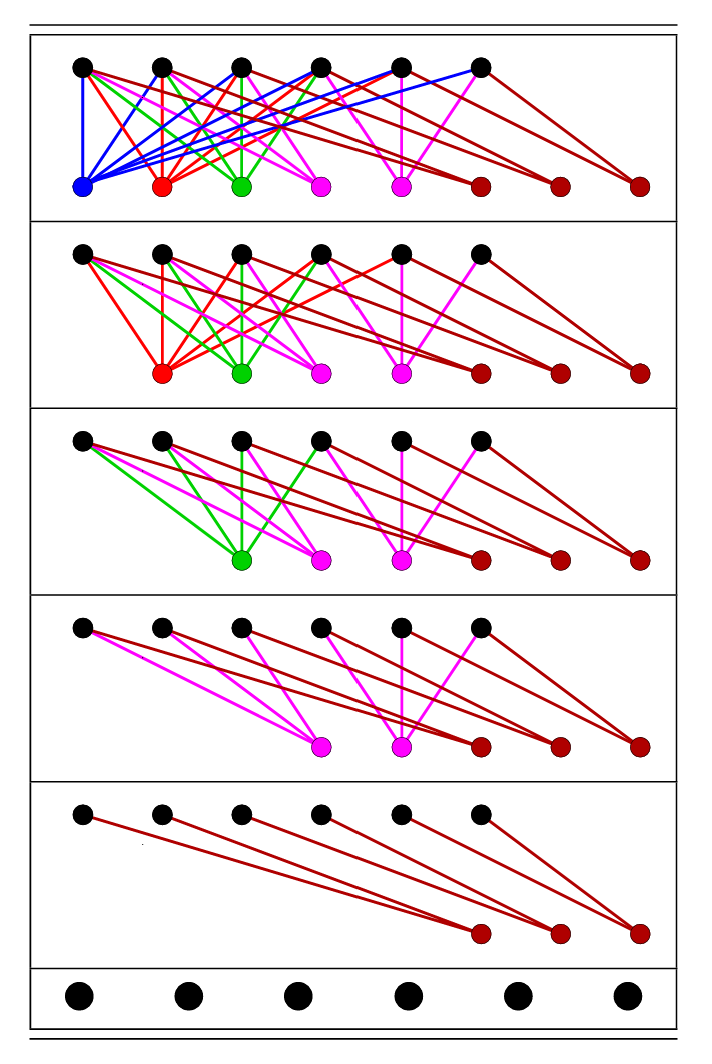
\includegraphics[width=0.5\textwidth]{GreedyVertexCover.png}  
    \end{figure}

    Let the first row of the graph be $n$ vertices, for the figure above it is $n = 6$. For the bottom row, for every $i$ from 2 to $n$, 
    we will have $\lfloor n/i \rfloor$ of degree $i$, each of them connected to distinct vertices in the top row. So in the above figure 
    we have 3 brown vertices of degree 2, 2 pink vertices of degree 3, 1 green, blue, red vertex of degree 4, 5, 6 respectively.

    Now let's see what vertices our greedy algorithm chooses. Firstly all vertices in the top row have degree at most $n-1$, as they can 
    be connected to at most 1 degree 2 vertex, degree 3 vertex, \dots, degree $n$ vertex. But the bottom row has a degree $n$ vertex right, 
    so it will be chosen first. Now after deleting this vertex and all its edges, the top row all have degree at most $n-2$, but the bottom 
    row has a degree $n-1$ vertex, so it will be chosen. We can actually inductively prove that only bottom row vertices will be chosen.

    Let's say the higher degrees from $k+1$ to $n$ have already been deleted from the bottom row, and you only have degree 2 to degree $k$.
    We can claim that the top row vertices all have degree at most $k-1$, as each of them is connected to atmost 1 vertex of degree 2, 1
    vertex of degree 3, \dots, 1 vertex of degree $k$. But the bottom row has vertices of degree $k$ so they'll get selected.

    Now how many vertices are we selecting? This is just 
    \begin{align*}
        \sum_{i=2}^n \lfloor n/i \rfloor &\geq \sum_{i=2}^n (n/i - 1) \\
        &= n \sum_{i=2}^n (1/i) - (n-1) \\
        &= n \sum_{i=1}^n (1/i) - n
    \end{align*}

    For the optimal vertex cover, we can just select the top row completely, which has $n$ vertices. So the approximation ratio is going 
    to be more than $\sum_{i=1}^n (1/i) - 1$, which is unbounded as the harmonic series diverges.

    \item Here's the problem, we have vertices $v_1$ to $v_n$ with some weights $w_1$ to $w_n$, we just want a vertex cover with minimum 
    sum of weights for all vertices selected. Our linear program for this is going to be as follows, we'll introduce new variables $x_1$
    to $x_n$ which kind of denote if the vertices are chosen or not. For every edge $v_i v_j$, we'll add a constraint $x_i + x_j \geq 1$
    which is like saying one of the vertices of each edge should be chosen. We want to minimize $\sum_i w_i x_i$ (obvious constraint is 
    $0 \leq x_i \leq 1$ for all $i$). And how we get an approximate solution from this linear program is by looking at the linear program's 
    optimal solution, and selecting all $v_i$'s which have $x_i$'s $\geq 1/2$. This is a valid vertex cover as if $x_i + x_j \geq 1$, 
    one of $x_i, x_j \geq 1/2$ which means every edge has a vertex selected.

    For the first line inequalities, it's obvious that the optimal solution can give a feasible solution to the linear program, by just
    making $x_i$'s 1 if $v_i$'s are selected in the optimal solution, and 0 otherwise. Since this satisfies all the constraints it's 
    feasible and will have weighted sum at least as much as the optimal solution of the linear program. Similarly the optimal vertex cover
    we get from the linear program is some vertex cover, so will have weighted sum at least as much as the optimal vertex cover, as the 
    optimal vertex cover by definition is the vertex cover with the least weighted sum.

    Now for the second line inequality. The key observation is that when we modify the optimal values for the linear program to get a
    vertex cover, we are not more than doubling the weighted sum. Each $x_i \geq 1/2$ is increased to 1, so at most the corresponding 
    term of the weighted sum is atmost doubled. The other $x_i$'s are made to 0, but even assuming that decrease never happens, the 
    overall weighted sum is atmost doubled. This means the vertex cover approximation algo is at most twice as bad as the lienar program
    optimal solution.

    \item For each of the edges $e_1$ to $e_n$, we keep variables $x_1$ to $x_n$ with the constraints $0 \leq x_i \leq 1$ for all $i$.
    For any 2 edges $e_i$ and $e_j$ which share a common vertex, $x_i + x_j \leq 1$. The linear program is to optimize $\sum_i w_i x_i$.
    Take the graph as a triangle with all the weights as 1. If we keep $x_1 = x_2 = x_3 = 1/2$, we get the maximum value of the linear 
    program as $3/2$, but obviously the maximum weight matching is only 1.

    \item Let there be $n$ loads, and $m$ processors, and let the optimal max load be $T^*$. There are 2 obvious inequalities related to 
    $T^*$. One is that $T^*$ is at least the max load, as it has to be placed somewhere. The other is that $T^*$ is at least the average 
    load on a processor i.e. $\left(\sum_i t_i\right) / m$ as the max load is at least the average load.
    Let us think about what's the load on a processor each time we place a load.

    \textbf{Case 1: }It's the first load for that processor, in this case the load on this process will be $\leq T^*$ for sure, as $T^*$ 
    is at least the max load.

    \textbf{Case 2: }There's at least one other load for that processor. Note that this has to be at least the ${(m+1)}^{th}$ load, as
    the greedy algo will place the first $m$ loads on different processes. But if there are that many loads, out the first $m+1$ loads, 
    2 of them have to be on the same processor in the optimal solution meaning $T^* \geq 2 t_{m+1}$. And the load we're placing right 
    is at most $t_{m+1}$ so current load $\leq T^*/ 2$. But what about the rest of the loads that were already there on the processor? 
    Our greedy algo has chosen the processor with the minimum load, so it's gonna be at most the average load at the moment, which is 
    at most the average load after placing all loads, which is at most $T^*$. So finally load on that processor $\leq T^*/2 + T^* = 
    3T^* / 2$.

    Turns out this approximation factor of 3/2 isn't tight, it can be proven that the greedy algo in descending order of loads actually 
    has an approximation factor of atmost 4/3.

    \item Our linear program will have variables $a_1, a_2, \dots, a_d, b, E$ ($E$ is an extra variable), and our goal is to minimize $E$.
    We will have $2n$ constraints, they are of the form $h(p_j) - l_j \leq E$, and $l_j - h(p_j) \leq E$, and we have this for all $j$ 
    from 1 to $n$. These are clearly linear equations once we expand $h(p_j)$ as $\sum_i a_i x_j^{(i)} + b$, but why does this work?
    The 2 constraints $h(p_j) - l_j \leq E$, and $l_j - h(p_j) \leq E$ basically say that $|h(p_j) - l_j| \leq E$, and if we want to
    combine the constraints for all $j$, it becomes $\max_j |h(p_j) - l_j| \leq E$. But in our linear program $E$ is free i.e.
    independent of all other parameters, but our objective is to minimize it. So in our optimal solution equality will be attained.
    
    \item Basically the same thing as the previous question, we'll have variables $a_{i,j}, 1 \leq i \leq j \leq d$ and $E$. Our goal
    is to minimize $E$. We'll have $2n$ constraints, which are $h(p_j) - l_j \leq E$, and $l_j - h(p_j) \leq E$, for all $j$ from 1 to 
    $n$. By the same logic, the equality will be attained in the optimal solution for $E$. 

    \item The obvious variables which will be in our linear program are $a_1, a_2, \dots, a_d, b$. But we'll add some extra variables.
    Here for each positively labelled point $p_j$ we introduce a variable $L_j$ in our linear program. We add the constraints that 
    $L_j \geq 1 - h(p_j)$, and $L_j \geq 0$. Similarly for every negatively labelled point $p_k$ we introduce a variable $L_k$ with 
    the constraints $L_k \geq 1 + h(p_k)$, and $L_k \geq 0$. Our objective in the linear program to minimize $\sum_j L_j + \sum_k L_k$.
    The optimal solution will have some equality for every $L_j$ and $L_k$ i.e $L_j = \max(1 - h(p_j), 0)$ and $L_k = \max(1 + h(p_k), 0)$.
    Because if not, they can be decreased more. This would mean the optimal value of our linear program is exactly the hinge loss.
    
    \item $X_i$ is a binary random variable, $E(X_i) = 1(1/i) + 0(1-1/i) = 1/i$. By law of expectation, $E(X) = E(\sum_i X_i) = 
    \sum_i E(X_i) = \sum_{i=1}^n 1/i$.

    \item Let $X$ be a random variable representing number of intersections. We know $E(X) \leq 2n$. From Markov's inequality, we 
    know that $P(X \geq 10n) \leq E(X)/10n \leq 2n/10n = 1/5$. So since $P(X \geq 10n) \leq 1/5$, $P(X < 10n) \geq 4/5$.

    \item No, it doesn't work, let's construct a counter example. We have the standard constraints $x \geq 0, y \geq 0$. We will 
    have $n$ different constraints $L_1, L_2, \dots, L_n$ where $L_i$ is $x/(n+1-i) + y/i \leq 1$. Say our objective function is 
    just to maximise $x$.

    Let's see how many times our intersection point is updated if the order of constraints we have is $i, i+1, \dots, n, 1, 2,
    \dots, i-1$. With just the first line, our optimal point is clearly $(n+1-i, 0)$. But this won't satisfy the second
    constraint, so our optimal point will get updated to $(n-i, 0)$. This pattern will continue till we add $L_n$, where our
    optimal point will finally become $(1,0)$ and then stop updating. So there are totally $n-i$ optimal point updates, and 
    each time we update we have to intersect the new line with all the previous lines. So we'll have $1 + 2 + \dots + (n-i)
    = (n-i)(n-i+1)/2$ intersection calculations. So let's now calculate the expected number of intersections.

    \begin{align*}
        \frac{1}{n} \sum_{i=1}^{n} \frac{(n-i)(n-i+1)}{2} &= \frac{1}{n} \sum_{i=1}^{n} \frac{(i)(i+1)}{2} \\
        &= \frac{1}{2n} \sum_{i=1}^{n} i^2 + \frac{1}{2n} \sum_{i=1}^{n} i \\
        &= \frac{(n)(n+1)(2n+1)}{12n} + \frac{(n)(n+1)}{4n} \\
        &= \frac{(n+1)(2n+1)}{12} + \frac{n+1}{4} \\
        &= \Theta(n^2)
    \end{align*}

    This is clearly not $O(n)$ like our previous calculations.

    \item Technically it isn't true in the 2D case that only 2 lines intersect at a corner of the feasible region. However, it actually
    doesn't matter, as even if it was the case, only 2 lines will be non-redundant. The one with the largest slope and the one with the 
    smallest slope are the only non-redundant lines, if their constraints are satisfied it would automatically satisfy all the constraints.

    But for the 3D case, you could have mutliple non-redundant constraints that a corner would satisfy. Take the top corner of a square 
    pyramid (since this solid has only plane faces, it can be the feasible region of a linear program). The corner is part of 4 planes, 
    and none of them are redundant. But for this question we will move the planes a bit such that no 4 planes intersect at a corner.

    After we introduce the $i^{th}$ constraint, the optimal point is going to be part of exactly 3 of the planes, so the probability that the final
    plane has the optimal point is $3/i$, so the probability the optimal point doesn't change is $1 - 3/i$. Suppose the optimal point 
    changes, we know that it's going to be part of the new plane, by a similar proof as in the 2D case.

    We have to now find the 2 other planes which intersect with this to give the optimal point. But since we know a plane where the
    optimal solution lies, we can just project every other plane onto this plane. We will get $i-1$ line constraints, for which we 
    have to find the optimal point, which is just our 2D problem. If we use our 2D algorithm for this, the expected time to get the 
    new point is $O(i)$.

    \item We change the constraints to $x_1, x_2, x_3, x_4 \geq 0$, and the equations are $x_1 + x_3 = 1, x_1 + x_2 + x_4 = 2$.
    In the simplex algorithm, we like to keep the basic variables on one side of equality, in the equations, so let's write it 
    as $x_3 = 1 - x_1$, and $x_4 = 2 - x_1 - x_2$. To find the values of the basic variables, you just look at the constant 
    term in each equation, the other variables are 0 anyway. So $x_3 = 1$ and $x_4 = 2$.

    Let's say we decide to increase $x_1$, and make it basic. The first equation can't increase $x_1$ more than 1, and the 
    second one can't increase $x_1$ more than 2. So we choose the first equation as it's a stronger constraint. Rewriting it,
    we get $x_1 = 1 - x_3$ and subbing this in the second equation, $x_4 = 1 + x_3 - x_2$. The point of this is that for each 
    equation, the LHS should be only basic variables and RHS should be only non-basic variables.
    The basic feasible solution is now $x_1 = 1, x_4 = 1$.
    Now we also have to rewrite our objective function with basic variables. So $2x_1 + x_2 = 2 - 2x_3 + x_2$. 

    Now we increase $x_2$. It's only part of the second equation, and it can be increased maximum to 1. So we rewrite it as 
    $x_2 = 1 + x_3 - x_4$. Our basic feasible solution is now $x_1 = 1, x_2 = 1$.
    Our objective function is now $2 - 2x+3 + (1 + x_3 - x_4) = 3 - x_3 - x_4$. Since all coefficients are negative now, we 
    stop.

    \item If we are at a point where our objective function is of the form $k - c_1 x_1 - c_2 x_2 - \dots - c_n x_n$, where 
    all the $c_i$'s and $x_i$'s are non negative, clearly the objective function can't be more than $k$. But we have actually
    achieved a value of $k$ as in our simplex method, the variables in the objective function are non-basic i.e. $0$. So 
    this has to be the optimal solution.

    \item If LP1 has a feasible solution, those same values of $x_i$'s will work for LP2, keeping all the $z_i$'s as $0$.
    Which would mean that the value of the objective function is also $0$. And we clearly can't do better, as the $z_i$'s 
    are supposed to be non negative. If LP2 has the optimal value as $0$, it has to be the case that all $z_i$'s are $0$ 
    in the optimal solution, as they are non-negative. But if they are $0$, the LHS of all equations are 0, which means 
    that the $x_i$'s satisfy LP1.
    
    \item Euclid's gcd algorithm gives us a way to find for any 2 integers $a, b$, some suitable $x, y$ such that $ax + by = \gcd(a,b)$.
    If $a$ is a non-zero number mod $p$, $gcd(a,p) = 1$ (can't be anything else, as $p$ has to be divisible by the gcd).
    This means we can find integers $x, y$ such that $ax + py = 1$ or $ax = 1 - py$. But this would just mean that $x$ 
    is the multiplicative inverse of $a$ as $ax$ is 1 plus a multiple of $p$.
    
    \item Firstly if the leading coefficient isn't 1, we can just divide the whole polynomial by that coefficient to make 
    it 1, clearly that doesn't change the roots. We'll prove this by induction, base case being constant polynomial obviously
    having $0$ roots, which is atmost $0$. Now take polynomial of degree $d$. If it has no roots, our statement is true.
    So assume it has a root $\alpha$. We can show that our polynomial is divisible by $x - \alpha$. If we do long division
    by the term $x - \alpha$, $P(x) = (x - \alpha)Q(x) + c$ ($c$ is the 0 degree remainder). Subbing $P(\alpha) = 0$, we get that 
    $c = 0$, so $P(x) = (x - \alpha)Q(x)$, where $Q(x)$ has to have degree $d-1$, with leading coefficient 1. We can now see 
    that any other root of $P(x)$ has to be a root of $Q(x)$. As if $P(\alpha') = 0$, $(\alpha' - \alpha)Q(\alpha') = 0$. As
    $\alpha' \neq \alpha$, $Q(\alpha') = 0$. But from our induction assumption, $Q(x)$ has atmost $d-1$ roots, which would mean 
    $P(x)$ has at most $d$ roots, which are the roots of $Q(x)$ along with $\alpha$.

    Actually the same idea holds if you work modulo $p$, where $p$ is prime. The starting of the proof is the same, let's 
    proceed from $P(x) = (x - \alpha)Q(x) + c$. $P(\alpha) = 0 \mod p$ means $c = 0 \mod p$, so since we're working modulo $p$, 
    we can ignore $c$. Now for any other root $\alpha'$ of $P(x)$, we get $(\alpha' - \alpha)Q(\alpha') = 0$, since $\alpha 
    \neq \alpha' \mod p$, we can actually multiply by its multplicative inverse of $(\alpha' - \alpha)$ on both sides to get that 
    $Q(\alpha') = 0$. So again, every other root of $P(x)$ is a root of $Q(x)$. By our induction assumption, since $Q(x)$ 
    has degree $d-1$ and leading coefficient 1, it has atmost $d-1$ roots. So $P(x)$ has atmost $d$ roots, which are the roots 
    of $Q(x)$ and $\alpha$.

    Note that we did use the fact that $p$ is prime while multiplying by the multiplicative inverse. The whole factor theorem
    idea only works if we have facts like $ab = 0$ implies $a = 0$ or $b = 0$. In fact if $p$ wasn't prime our statement is 
    false. For example $x^2 - 1 = 0 \mod 8$ has 4 distinct roots - $1, 3, 5, 7$.

    \item Assuming none of the points have the same x coordinate, and the question means degree atmost $d$.
    
    It's easy to prove that there can be atmost 1 curve. Assume there are 2 distinct curves of degree atmost $d$ which pass through
    all the points. But then their polynomial difference would evaluate to 0 at all these points. This would mean we have a polynomial
    of degree atmost $d$ has $d+1$ roots, which isn't possible unless the polynomial is literally 0, meaning the curves were
    the same all along.

    Now to show that there exists such a curve. Let the points it has to pass through be the following:
    $(x_1, y_1), (x_2, y_2), \dots, (x_d, y_d)$. We'll try to find a polynomial of degree atmost $d-1$ which passes through all 
    these points.

    Think about the term $c_1(x - x_2)(x - x_3)\dots(x - x_d)$ where $c_1$ is some parameter. By tweaking $c_1$, note that the value 
    of the term changes at only $x = x_1$ but stays equal to 0 at every other point $x_2, x_3, \dots, x_d$. In fact if we keep 
    \[c_1  = \frac{y_1}{\prod_{j = 2}^n (x_1 - x_j)} \]
    the term will evaluate to $y_1$ at $x_1$. If we just add such terms which only affect the values at $x_2, \dots, x_d$ we'll be 
    done. So we have the following equation for $P(x)$:

    \[P(x) = \sum_{i=1}^d c_i \left(\prod_{j \neq i} (x - x_j)\right) = \sum_{i=1}^d \frac{y_i}{\prod_{j \neq i} (x_i - x_j)} \left(\prod_{j \neq i} (x - x_j)\right) \]

    If we think about it, when we evaluate $P(x_i)$, the $i^{th}$ term is the only non-zero term in the summation, and $c_i$ has been 
    chosen specifically such that $P(x_i) = y_i$. This is clearly a polynomial with degree atmost $d-1$ which satisfies our conditions
    so we have proven our claim. This polynomial construction is known as Lagrange interpolation.
    
    \item Using the idea above, let's construct $P(x)$ like the following:

    \[ P(x) = c_1(x-1)(x-2)(x-5) + c_2(x)(x-2)(x-5)+ c_3(x)(x-1)(x-5) + c_4(x)(x-1)(x-2) \]

    By substituting $x = 0,1,2,5$, we get $c_1 = -3/10, c_2 = 1/2, c_3 = -1/3, c_4 = 1/60$. So that's our 3rd degree polynomial.

    \item If we choose some random 68 points, we know that a maximum of 32 can be modified points, so we'll get a minimum of 36 unaltered 
    points. There's only a unique curve of degree at most 35 passing through these 36 points, and we know our original curve that 
    we started has degree atmost 35 and passes through these 36 points. So our original curve is the only curve which passes 
    through these 36 points, and hence has to be the only curve which passes through the 68 points.
    
\end{enumerate}
\end{document}